\documentclass[twoside,11pt]{article}

% +
%  Name:
%     sun230.tex

%  Purpose:
%     SUN documentation for ORAC-DR overview (SUN/230)

%  Authors:
%     Frossie Economou (JACH)
%     Tim Jenness (JACH)

%  Copyright:
%     Copyright (C) 1997-2000 Particle Physics and Astronomy
%     Research Council. All Rights Reserved.

%  Notes:
%     The final SUN is generated automatically from POD. Once the
%     latex is generated the following changes are required:
%     - Replace ORAC-DR with \oracdr\
%     - Remove any junk from the start and end of each pod section.
%       Usually involves removing everything up to and including the
%       DESCRIPTION section declaration, leaving the description in place
%       as a section introduction. Remove COPYRIGHT, AUTHOR and REVISION
%       sections.
%     - Remove % from end of pod2latex generated \item commands (and
%       \index commands) since they are not needed
%       and they ruin the star2html conversion.
%     - Usually replace 'this document' with 'this section'
%     - Add xlabels to all sections/subsections
%     - References to CGS4DR should be replaced with \cgsdr\
%     - References to GAIA should be replaced with \gaia\
%     - References to GWM should be replaced with \gwm\
%     - References to Kappa should be replaced with \Kappa\
%     - References to KAPVIEW should be replaced with \kapview\
%     - Replace P4 with \textsc{p4}
%     - Replace (C) with \copyright
%     - Replace SUN/231 and SUN/232 references with real xrefs


%  History:
%     $Log$
%     Revision 1.5  2000/02/09 20:18:12  timj
%     Correct stardocnumber to .1 rather than .0
%
%     Revision 1.4  2000/02/08 19:42:40  timj
%     Correct missing xlabel
%
%     Revision 1.3  2000/02/08 04:41:09  timj
%     Fixes to documentation required by Starlink for release of V1.0-0
%
%     Revision 1.2  2000/02/03 10:48:52  timj
%     Fix credits after input from UKATC
%
%     Revision 1.1.1.1  2000/02/03 09:44:59  timj
%     first starlink docs
%

%  Revision:
%     $Id$

% -

% ? Specify used packages
\usepackage{graphicx}        %  Use this one for final production.
\usepackage{times}
% \usepackage[draft]{graphicx} %  Use this one for drafting.
% ? End of specify used packages

\pagestyle{myheadings}

% -----------------------------------------------------------------------------
% ? Document identification
% Fixed part
\newcommand{\stardoccategory}  {Starlink User Note}
\newcommand{\stardocinitials}  {SUN}
\newcommand{\stardocsource}    {sun\stardocnumber}

% Variable part - replace [xxx] as appropriate.
\newcommand{\stardocnumber}    {230.1}
\newcommand{\stardocauthors}   {Frossie Economou, Tim Jenness,\\ Malcolm Currie, Andy Adamson\\
Joint Astronomy Centre, Hilo, Hawaii}
\newcommand{\stardocdate}      {1 Feb 2000}
\newcommand{\stardoctitle}     {ORAC-DR: Overview and General Introduction}
\newcommand{\stardocversion}   {1.0-0}
\newcommand{\stardocmanual}    {}

\newcommand{\stardocabstract}  {\textsc{orac-dr} is a general purpose
automatic data reduction pipeline environment. It currently supports data
reduction for the United Kingdom Infrared Telescope (UKIRT) instruments UFTI
and IRCAM, and for the James Clerk Maxwell Telescope (JCMT) instrument
SCUBA. This document describes the general pipeline environment. For specific
information on how to reduce the data for a particular instrument, please
consult the appropriate \textsc{orac-dr} instrument guide.}

% ? End of document identification
% -----------------------------------------------------------------------------

% +
%  Name:
%     sun.tex
%
%  Purpose:
%     Template for Starlink User Note (SUN) documents.
%     Refer to SUN/199
%
%  Authors:
%     AJC: A.J.Chipperfield (Starlink, RAL)
%     BLY: M.J.Bly (Starlink, RAL)
%     PWD: Peter W. Draper (Starlink, Durham University)
%
%  History:
%     17-JAN-1996 (AJC):
%        Original with hypertext macros, based on MDL plain originals.
%     16-JUN-1997 (BLY):
%        Adapted for LaTeX2e.
%        Added picture commands.
%     13-AUG-1998 (PWD):
%        Converted for use with LaTeX2HTML version 98.2 and
%        Star2HTML version 1.3.
%     {Add further history here}
%
% -

\newcommand{\stardocname}{\stardocinitials /\stardocnumber}
\markboth{\stardocname}{\stardocname}
\setlength{\textwidth}{160mm}
\setlength{\textheight}{230mm}
\setlength{\topmargin}{-2mm}
\setlength{\oddsidemargin}{0mm}
\setlength{\evensidemargin}{0mm}
\setlength{\parindent}{0mm}
\setlength{\parskip}{\medskipamount}
\setlength{\unitlength}{1mm}

% -----------------------------------------------------------------------------
%  Hypertext definitions.
%  ======================
%  These are used by the LaTeX2HTML translator in conjunction with star2html.

%  Comment.sty: version 2.0, 19 June 1992
%  Selectively in/exclude pieces of text.
%
%  Author
%    Victor Eijkhout                                      <eijkhout@cs.utk.edu>
%    Department of Computer Science
%    University Tennessee at Knoxville
%    104 Ayres Hall
%    Knoxville, TN 37996
%    USA

%  Do not remove the %begin{latexonly} and %end{latexonly} lines (used by 
%  LaTeX2HTML to signify text it shouldn't process).
%begin{latexonly}
\makeatletter
\def\makeinnocent#1{\catcode`#1=12 }
\def\csarg#1#2{\expandafter#1\csname#2\endcsname}

\def\ThrowAwayComment#1{\begingroup
    \def\CurrentComment{#1}%
    \let\do\makeinnocent \dospecials
    \makeinnocent\^^L% and whatever other special cases
    \endlinechar`\^^M \catcode`\^^M=12 \xComment}
{\catcode`\^^M=12 \endlinechar=-1 %
 \gdef\xComment#1^^M{\def\test{#1}
      \csarg\ifx{PlainEnd\CurrentComment Test}\test
          \let\html@next\endgroup
      \else \csarg\ifx{LaLaEnd\CurrentComment Test}\test
            \edef\html@next{\endgroup\noexpand\end{\CurrentComment}}
      \else \let\html@next\xComment
      \fi \fi \html@next}
}
\makeatother

\def\includecomment
 #1{\expandafter\def\csname#1\endcsname{}%
    \expandafter\def\csname end#1\endcsname{}}
\def\excludecomment
 #1{\expandafter\def\csname#1\endcsname{\ThrowAwayComment{#1}}%
    {\escapechar=-1\relax
     \csarg\xdef{PlainEnd#1Test}{\string\\end#1}%
     \csarg\xdef{LaLaEnd#1Test}{\string\\end\string\{#1\string\}}%
    }}

%  Define environments that ignore their contents.
\excludecomment{comment}
\excludecomment{rawhtml}
\excludecomment{htmlonly}

%  Hypertext commands etc. This is a condensed version of the html.sty
%  file supplied with LaTeX2HTML by: Nikos Drakos <nikos@cbl.leeds.ac.uk> &
%  Jelle van Zeijl <jvzeijl@isou17.estec.esa.nl>. The LaTeX2HTML documentation
%  should be consulted about all commands (and the environments defined above)
%  except \xref and \xlabel which are Starlink specific.

\newcommand{\htmladdnormallinkfoot}[2]{#1\footnote{#2}}
\newcommand{\htmladdnormallink}[2]{#1}
\newcommand{\htmladdimg}[1]{}
\newcommand{\hyperref}[4]{#2\ref{#4}#3}
\newcommand{\htmlref}[2]{#1}
\newcommand{\htmlimage}[1]{}
\newcommand{\htmladdtonavigation}[1]{}

\newenvironment{latexonly}{}{}
\newcommand{\latex}[1]{#1}
\newcommand{\html}[1]{}
\newcommand{\latexhtml}[2]{#1}
\newcommand{\HTMLcode}[2][]{}

%  Starlink cross-references and labels.
\newcommand{\xref}[3]{#1}
\newcommand{\xlabel}[1]{}

%  LaTeX2HTML symbol.
\newcommand{\latextohtml}{\LaTeX2\texttt{HTML}}

%  Define command to re-centre underscore for Latex and leave as normal
%  for HTML (severe problems with \_ in tabbing environments and \_\_
%  generally otherwise).
\renewcommand{\_}{\texttt{\symbol{95}}}

% -----------------------------------------------------------------------------
%  Debugging.
%  =========
%  Remove % on the following to debug links in the HTML version using Latex.

% \newcommand{\hotlink}[2]{\fbox{\begin{tabular}[t]{@{}c@{}}#1\\\hline{\footnotesize #2}\end{tabular}}}
% \renewcommand{\htmladdnormallinkfoot}[2]{\hotlink{#1}{#2}}
% \renewcommand{\htmladdnormallink}[2]{\hotlink{#1}{#2}}
% \renewcommand{\hyperref}[4]{\hotlink{#1}{\S\ref{#4}}}
% \renewcommand{\htmlref}[2]{\hotlink{#1}{\S\ref{#2}}}
% \renewcommand{\xref}[3]{\hotlink{#1}{#2 -- #3}}
%end{latexonly}
% -----------------------------------------------------------------------------
% ? Document specific \newcommand or \newenvironment commands.

\def\C++{{\rm C\kern-.05em\raise.3ex\hbox{\footnotesize ++}}}
\newcommand{\underscore}{\_}
\newcommand{\oracdr}{\textsc{orac-dr}}

% For HTML redefine hfil since latex2html does not understand it
\html{\renewcommand{\hfil}{ }}

\newcommand{\recipe}[1]{{\small\textsf{#1}}}
\newcommand{\primitive}[1]{{\small\texttt{#1}}}

\newcommand{\Kappa}{\xref{{\textsc{Kappa}}}{sun95}{}}
\newcommand{\kapview}{\textsc{kapview}}
\newcommand{\gaia}{\xref{{\textsc{Gaia}}}{sun214}{}}
\newcommand{\cgsdr}{\xref{{\textsc{cgs4dr}}}{sun27}{}}
\newcommand{\gwm}{\xref{\textsc{gwm}}{sun219}{}}

% ? End of document specific commands
% -----------------------------------------------------------------------------
%  Title Page.
%  ===========
\renewcommand{\thepage}{\roman{page}}
\begin{document}
\thispagestyle{empty}

%  Latex document header.
%  ======================
\begin{latexonly}
   CCLRC / \textsc{Rutherford Appleton Laboratory} \hfill \textbf{\stardocname}\\
   {\large Particle Physics \& Astronomy Research Council}\\
   {\large Starlink Project\\}
   {\large \stardoccategory\ \stardocnumber}
   \begin{flushright}
   \stardocauthors\\
   \stardocdate
   \end{flushright}
   \vspace{-4mm}
   \rule{\textwidth}{0.5mm}
   \vspace{5mm}
   \begin{center}
   {\Huge\textbf{\stardoctitle \\ [2.5ex]}}
   {\LARGE\textbf{\stardocversion \\ [4ex]}}
   {\Huge\textbf{\stardocmanual}}
   \end{center}
   \vspace{5mm}

% ? Add picture here if required for the LaTeX version.
%   e.g. \includegraphics[scale=0.3]{filename.ps}
\begin{center}

\includegraphics[width=1.0in]{sun230_logo.eps}
\end{center}
% ? End of picture

% ? Heading for abstract if used.
   \vspace{10mm}
   \begin{center}
      {\Large\textbf{Abstract}}
   \end{center}
% ? End of heading for abstract.
\end{latexonly}

%  HTML documentation header.
%  ==========================
\begin{htmlonly}
   \xlabel{}
   \begin{rawhtml} <H1> \end{rawhtml}
      \stardoctitle\\
      \stardocversion\\
      \stardocmanual
   \begin{rawhtml} </H1> <HR> \end{rawhtml}

% ? Add picture here if required for the hypertext version.
%   e.g. \includegraphics[scale=0.7]{filename.ps}

\includegraphics[width=1.0in]{sun230_logo.eps}
% ? End of picture

   \begin{rawhtml} <P> <I> \end{rawhtml}
   \stardoccategory\ \stardocnumber \\
   \stardocauthors \\
   \stardocdate
   \begin{rawhtml} </I> </P> <H3> \end{rawhtml}
      \htmladdnormallink{CCLRC / Rutherford Appleton Laboratory}
                        {http://www.cclrc.ac.uk} \\
      \htmladdnormallink{Particle Physics \& Astronomy Research Council}
                        {http://www.pparc.ac.uk} \\
   \begin{rawhtml} </H3> <H2> \end{rawhtml}
      \htmladdnormallink{Starlink Project}{http://www.starlink.rl.ac.uk/}
   \begin{rawhtml} </H2> \end{rawhtml}
   \htmladdnormallink{\htmladdimg{source.gif} Retrieve hardcopy}
      {http://www.starlink.rl.ac.uk/cgi-bin/hcserver?\stardocsource}\\

%  HTML document table of contents. 
%  ================================
%  Add table of contents header and a navigation button to return to this 
%  point in the document (this should always go before the abstract \section). 
  \label{stardoccontents}
  \begin{rawhtml} 
    <HR>
    <H2>Contents</H2>
  \end{rawhtml}
  \htmladdtonavigation{\htmlref{\htmladdimg{contents_motif.gif}}
        {stardoccontents}}

% ? New section for abstract if used.
  \section{\xlabel{abstract}Abstract}
% ? End of new section for abstract
\end{htmlonly}

% -----------------------------------------------------------------------------
% ? Document Abstract. (if used)
%  ==================
\stardocabstract
% ? End of document abstract
% -----------------------------------------------------------------------------
% ? Latex document Table of Contents (if used).
%  ===========================================
  \newpage
  \begin{latexonly}
    \setlength{\parskip}{0mm}
    \tableofcontents
    \setlength{\parskip}{\medskipamount}
    \markboth{\stardocname}{\stardocname}
  \end{latexonly}
% ? End of Latex document table of contents
% -----------------------------------------------------------------------------
\cleardoublepage
\renewcommand{\thepage}{\arabic{page}}
\setcounter{page}{1}

% ? Main text

%% ORACDRDOC_HOWTO:Introduction
% LaTeX document produced by pod2latex from "Introduction.pod".
% The followings need be defined in the preamble of this document:
%\def\C++{{\rm C\kern-.05em\raise.3ex\hbox{\footnotesize ++}}}
%\def\underscore{\leavevmode\kern.04em\vbox{\hrule width 0.4em height 0.3pt}}
%\setlength{\parindent}{0pt}

\section{Introduction\xlabel{introduction}}

This document gives a general introduction to the pipeline, what it
does and what it will not do. For information on instrument
specific functions, see \xref{SUN/231}{sun231}{} for SCUBA and
\xref{SUN/232}{sun232}{} for IRCAM and UFTI.

\subsection*{What it is}
\index{What it is}

The \oracdr\ data reduction system is intended to be a pipeline reducer
for incoming data. It is in use for online data reduction at UKIRT and
JCMT for a variety of instruments. There are a number of differences
between the \oracdr\ method of reduction and other systems currently in
use and observers should not expect \oracdr\ to behave or be used in
the same way as those systems.

Firstly, \oracdr\ aims to reduce data to a point where its quality can
be assessed; it will not generally produce publication-quality results
(though in certain circumstances it may do).  Secondly, although
\oracdr\ also works offline, it is expected that observers will use
their own preferred data reduction package if they wish to work
interactively work on their data. The rest of this document summarizes
and accounts for the operational differences between the pipeline and
existing packages.

\subsection*{It pipes, therefore it is}
\index{It pipes, therefore it is}

This is crucial. Everything else about the package is clear once this
is grasped. This is not a reduction package like \cgsdr; it is a
reduction black box which knows the incoming data types (by their
headers) and transparently applies a reduction recipe to them. There
is nothing preventing you from running three simultaneous instances of
the pipeline, for example to (i) reduce the incoming data in real
time, (ii) re-reduce a previous group of files using a different
reduction recipe and (iii) reduce and file a single previous
observation as a dark. You do this by running three versions of
oracdr, using the command-line switches to alter their behavior
(recipe, start and end observation numbers to process, graphics
options, etc.). Each instance of the pipeline will go through the
required files (existing ones or files just arriving on disk as
specified on the command line) and reduce them. Once its remit of
reduction is complete, it will exit.

\subsection*{Control}
\index{Control}

The behavior of \oracdr\ is entirely controlled by the command line
options entered at startup. From that point on, the system either
takes its reduction recipe instructions from the file headers (this is
the default) or uses a hardwired recipe given on the command line
itself. The recipe is, in fact, the only allowed parameter on the
command line --- all the rest are options. Once you start an instance of
oracdr up, there is no further control over it; this is a considerable
change from the situation with \cgsdr, for example, where the same
package remains up once you start it, and changes are made within the
package. Corollary: if the pipeline fails to find a required
calibration frame, for example, the only logical thing for it to do is
exit cleanly, telling you why it did so. There is no control from
within the pipeline. Note that once the full ORAC system is available,
there will be plenty of pre-checking that your calibration frames will
indeed exist and be appropriate. Until that point, the behavior of
the system is logical if you understand the underlying philosophy and
do not expect to be able to control the pipeline in real time.


%% ORACDRDOC_HOWTO:Jargon
% LaTeX document produced by pod2latex from "Jargon.pod".
% The followings need be defined in the preamble of this document:
%\def\C++{{\rm C\kern-.05em\raise.3ex\hbox{\footnotesize ++}}}
%\def\underscore{\leavevmode\kern.04em\vbox{\hrule width 0.4em height 0.3pt}}
%\setlength{\parindent}{0pt}

\section{Jargon\xlabel{jargon}}
\index{JARGON}

This section describes some of the terms commonly used in
the \oracdr\ documentation.

\subsection*{What it says}
\index{What it says}

\oracdr\ is a data-driven data pipeline that uses recipes and
primitives to drive external algorithm engines to perform actual data
reduction.

\subsection*{What it means}
\index{What it means}

\begin{description}

\item[pipeline]
\index{pipeline@pipeline}
\hfil\\
Software that runs without external intervention, taking raw data on
one end and producing reduced data in the other.

\item[data-driven]\index{data-driven@data-driven}\hfil\\
Software that does nothing until data arrives, and then looks to 
the data and not the user for data reduction information.

\item[recipe]
\index{recipe@recipe}
\hfil\\
A file containing a list of individual data reduction steps. 

\item[primitive]
\index{primitive@primitive}
\hfil\\
A file containing code performing a meaningful data reduction step

\item[engine]
\index{engine@engine}
\hfil\\
An external package (e.g. a Starlink task) that performs a certain
algorithmic step (e.g. addition).

\end{description}

\begin{figure}
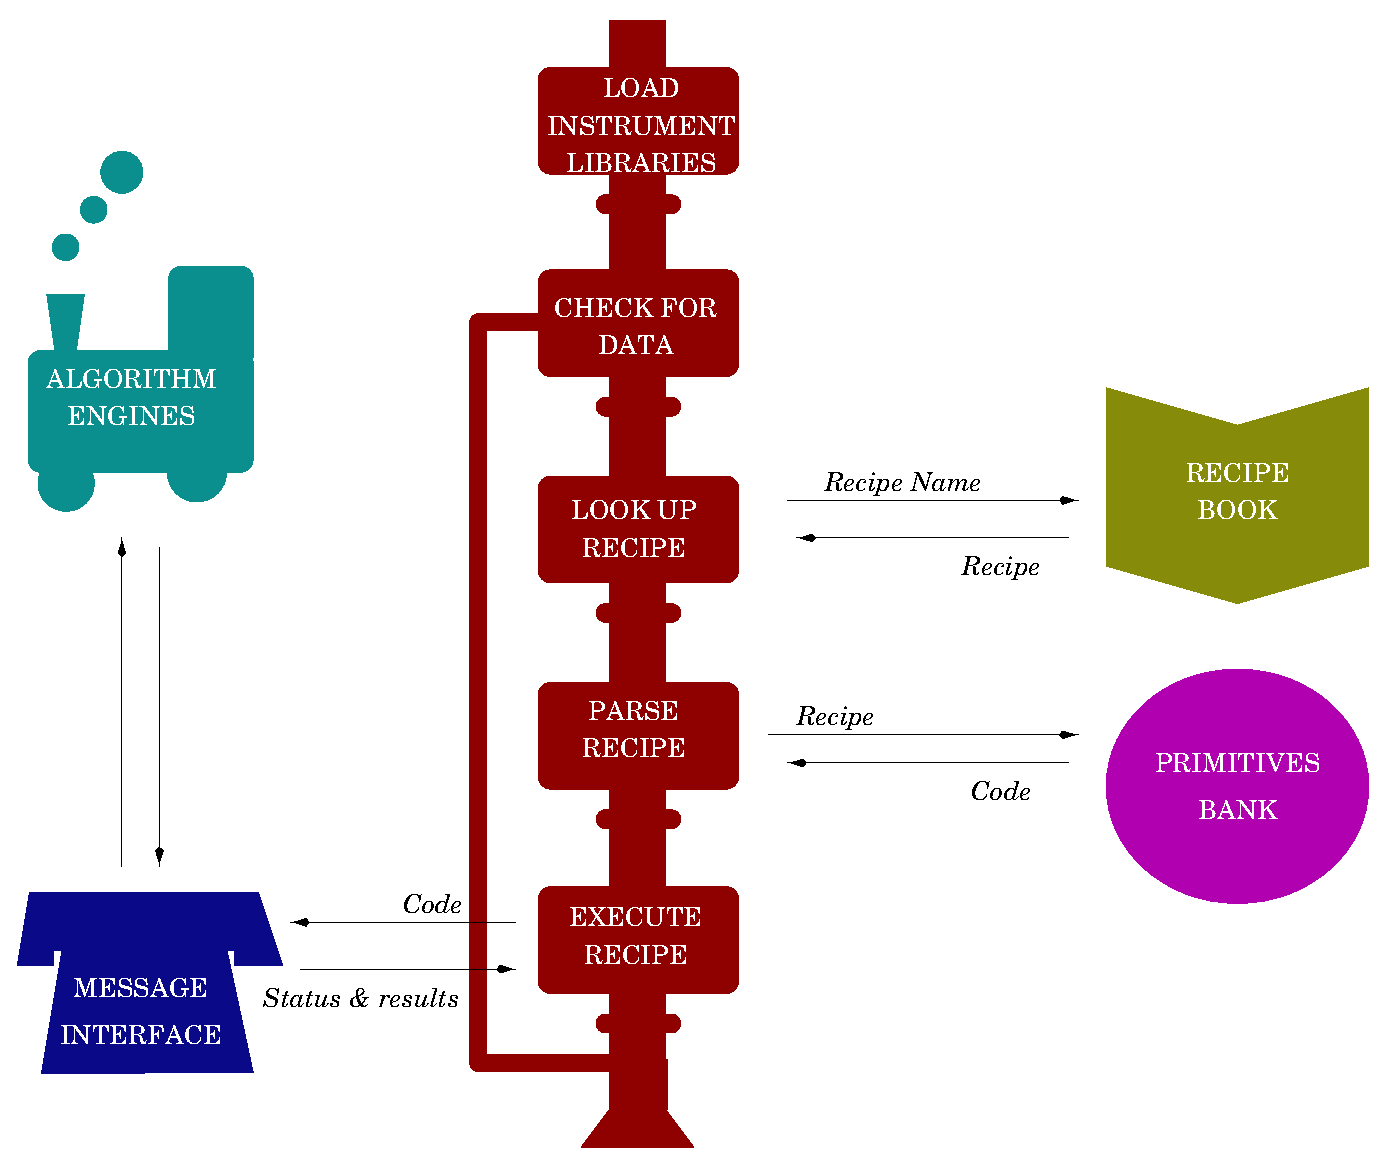
\includegraphics[width=\textwidth]{sun230_train.eps}
\caption{What happens in \oracdr}
\end{figure}



%% ORACDRDOC_HOWTO:SettingUp
% LaTeX document produced by pod2latex from "SettingUp.pod".
% The followings need be defined in the preamble of this document:
%\def\C++{{\rm C\kern-.05em\raise.3ex\hbox{\footnotesize ++}}}
%\def\underscore{\leavevmode\kern.04em\vbox{\hrule width 0.4em height 0.3pt}}
%\setlength{\parindent}{0pt}

\section{Setting Up\xlabel{setting_up}}
\index{SETTINGUP}

This section describes how to set up the \oracdr\ software for your
environment. \oracdr\ requires \texttt{tcsh} for full functionality
from the system setup. If
 \texttt{tcsh} is not available the startup scripts (\texttt{oracdr\_ufti} etc)
 will not set the specified UT date (the argument is ignored). In this case
 the \texttt{ORAC\_DATA\_IN} and \texttt{ORAC\_DATA\_OUT} environment
 variables must be set up explicitly.  Additionally, the \texttt{oracdr}
 command must include the `\textbf{-ut}' option as specified in the
 \texttt{oracdr} documentation.

\subsection*{The short way (Starlink and JAC users only)}
\index{short way (Starlink and JAC users only)}

\begin{itemize}

\item
If your data conforms to the directory naming convention of the
instrument, type:
\begin{verbatim}
 setenv ORAC_DATA_ROOT <root data directory>
 oracdr_<instrument> YYYYMMDD
\end{verbatim}

You can set up this variable by hand or in your own login script
{\bf before} running the oracdr instrument setup script.

For example, the naming convention for UFTI data is
{\tt ufti\char`\_data/YYYYMMDD/raw/} for the location of raw data and
{\tt ufti\char`\_data/YYYYMMDD/reduced/} for the location of reduced data. You can
set {\tt ORAC\char`\_DATA\char`\_ROOT} to the directory in which the UT directory is
found. So if your raw UFTI data is in
{\tt /home/user/data/UKIRT/ufti\char`\_data/YYYYMMDD/raw/} you should type:
\begin{verbatim}
 setenv ORAC_DATA_ROOT /home/user/data/UKIRT/
 oracdr_ufti
 oracdr [-options] [RECIPE]
\end{verbatim}

in order to reduce your UFTI data.

\item
If your raw and reduced data are in arbitrary directories, type:
\begin{verbatim}
 oracdr_instrument <YYYYMMDD>
 setenv ORAC_DATA_IN <raw data directory>
 setenv ORAC_DATA_OUT <reduced data directory>
\end{verbatim}

e.g. 
\begin{verbatim}
 oracdr_ufti 19990602
 setenv ORAC_DATA_IN /home/user/data/patt99/raw/
 setenv ORAC_DATA_OUT /scratch/user
 oracdr [-options] [RECIPE]
\end{verbatim}

\end{itemize}

Note that \oracdr\ works exclusively in {\tt ORAC\char`\_DATA\char`\_OUT}, irrespective of
what your current directory is when you invoke it.

\subsection*{The long way}
\index{long way}

\oracdr\ uses a number of environment variables for configuration. If
you are using a non-Starlink non-JAC installation of \oracdr, please
consult the {\em ShellVariables\/} manpage (see appendix) for the complete set of
variables and their meaning.

%% ORACDRDOC_HOWTO:Components
% LaTeX document produced by pod2latex from "Components.pod".
% The followings need be defined in the preamble of this document:
%\def\C++{{\rm C\kern-.05em\raise.3ex\hbox{\footnotesize ++}}}
%\def\underscore{\leavevmode\kern.04em\vbox{\hrule width 0.4em height 0.3pt}}
%\setlength{\parindent}{0pt}

\section{Components\xlabel{components}}
\index{COMPONENTS}

This section describes the executables that form part of the \oracdr\
distribution.

\subsection*{Set up scripts}
\index{Set up scripts}

These are the commands you have to type to set up \oracdr\ for the various
supported instruments.

\begin{description}

\item[{\tt oracdr\char`\_ircam}]
\index{oracdr_ircam@{\tt oracdr\char`\_ircam}}
\hfil\\
Sets up for the data reduction of IRCAM, the UKIRT Infrared Camera.

\item[{\tt oracdr\char`\_scuba}]
\index{oracdr_scuba@{\tt oracdr\char`\_scuba}}
\hfil\\
Sets up for the data reduction of SCUBA, the JCMT Submillimetre Common
User Bolometer Array.

\item[{\tt oracdr\char`\_ufti}]
\index{oracdr_ufti@{\tt oracdr\char`\_ufti}}
\hfil\\
Sets up for the data reduction of UFTI (the UKIRT Fast Track Imager)

\end{description}

Support for the CGS4 (the UKIRT Cooled Grating Spectrometer) and
Michelle (the UKIRT/Gemini Mid-Infrared Echelle spectrometer) is
also planned.

\subsection*{Executables}
\index{Executables}

\begin{description}

\item[{\tt oracdr}]
\index{oracdr@{\tt oracdr}}
\hfil\\
Runs the pipeline. For more information see the {\em oracdr\/} manpage

\item[{\tt oracman}]
\index{oracman@{\tt oracman}}
\hfil\\
Displays man-page information for all \oracdr\ executables, recipes,
primitives and how-to guides. Type:
\begin{verbatim}
 oracman <foo>
\end{verbatim}

for documentation, e.g.
\begin{verbatim}
 oracman oracdr
 oracman ARRAY_TESTS
 oracman _SUBTRACT_DARK_
 oracman DisplaySystem
\end{verbatim}

\item[{\tt oracdisp}]
\index{oracdisp@{\tt oracdisp}}
\hfil\\
Sets up the X display configuration tool. For more information on
{\tt oracdisp} and the display system see the {\em oracdisp\/} manpage and the {\em DisplaySystem\/} manpage

\item[{\tt oracdr\char`\_nuke}]
\index{oracdr_nuke@{\tt oracdr\char`\_nuke}}
\hfil\\
Kills {\tt oracdr}, any related processes (including any Starlink
processes), and clears shared memory owned by the user. Useful if
something happens to cause \oracdr\ to hang. See the {\em oracdr\underscore{}nuke\/} manpage

\end{description}

% LaTeX document produced by pod2latex from "oracdr.pod".
% The followings need be defined in the preamble of this document:
%\def\C++{{\rm C\kern-.05em\raise.3ex\hbox{\footnotesize ++}}}
%\def\underscore{\leavevmode\kern.04em\vbox{\hrule width 0.4em height 0.3pt}}
%\setlength{\parindent}{0pt}

\section{ORACDR\xlabel{oracdr}}
\index{ORACDR}

{\tt oracdr} is the actual \oracdr\ data reduction pipeline. 
This document describes the command line options that
can be used to modify the pipeline operation.

\subsection*{Arguments}
\index{Arguments}

The following argument  is  supported:

\begin{itemize}

\item{\bf RECIPE}
\index{RECIPE@RECIPE}
\hfil\\
By default, \oracdr\ looks in the file header for the name of the
recipe to be used on the data. If you specify the name of a recipe on
the command line, it will override the one specified in the
header. This override recipe is used for all data files regardless of
header contents or observation mode, so make sure you only only apply
it to appropriate data frames.

\end{itemize}

\subsection*{Options}
\index{Options}

All \oracdr\ behaviour is controlled by the option
switches. These options may be abbreviated to a unique substring. It
is via command line switches that you (for example) control the range
of file numbers to be reduced, force the system to use a particular
calibration file when reducing (e.g. to try a different flat
exposure). This list needs to be read thoroughly by anyone wanting to
use the system.

\subsubsection*{General Options}
\index{General Options}

\begin{itemize}

\item{\bf -help}
\index{-help@-help}
\hfil\\
List help text. This prints a summary of this document.

\item{\bf -version}
\index{-version@-version}
\hfil\\
Print the version number.

\item{\bf -verbose}
\index{-verbose@-verbose}
\hfil\\
Print messages from the Starlink engines (rather than just \oracdr\
messages).

\item{\bf -debug}
\index{-debug@-debug}
\hfil\\
Log debug messages to file {\tt ORACDR.DEBUG} in {\tt \$ORAC\char`\_DATA\char`\_OUT}.

\item{\bf -warn}
\index{-warn@-warn}
\hfil\\
Turn on perl level warning messages ({\tt perl -w}). This should be
used for debugging only. If {\tt -verbose} is also true then full 
perl diagnostics are turned on (see the {\em diagnostics\/} manpage for more information
on this perl pragma).

\item{\bf -beep}
\index{-beep@-beep}
\hfil\\
Make as much noise as possible over errors and pipeline exit.
Default is not to beep.

\end{itemize}

\subsubsection*{Windows and output}
\index{Windows and output}

\begin{itemize}

\item{\bf -nodisplay}
\index{-nodisplay@-nodisplay}
\hfil\\
Do not launch the display system. No data will be displayed and \gwm,
\gaia\ etc. windows will not be launched.

\item{\bf -log s}
\index{-log s@-log s}
\hfil\\
Log to terminal screen (standard out)

\item{\bf -log f}
\index{-log f@-log f}
\hfil\\
Log to a file. The logfile is called {\tt .oracdr\char`\_NNNN.log} where NNNN 
is the current process ID. It is written to {\tt \$ORAC\char`\_DATA\char`\_OUT} and is 
a hidden file.

\item{\bf -log x}
\index{-log x@-log x}
\hfil\\
Log to an Xwindow. Has the advantage that warnings and errors are
written to different, independently scrollable windows.

\end{itemize}

The three log options can be combined. The default is {\tt -log sx}

To run \oracdr\ using output only within the xterm that you used
to invoke it in, use {\tt -nodisplay -log s}. This is the fastest way
to run the pipeline if you are not interested in visually
inspecting the data as it is being reduced.

\subsubsection*{Observation numbers}
\index{Observation numbers}

\begin{itemize}

\item{\bf -from}
\index{-from@-from}
\hfil\\
Number of first observation.

\item{\bf -to}
\index{-to@-to}

Number of last observation.

\item{\bf -list}
\index{-list@-list}
\hfil\\
Comma separated list of observation {\em numbers\/}. Colons indicate a range.
For example, `1,2,4:6,10' means 1,2,4,5,6,10.

\end{itemize}

\subsubsection*{UT date}
\index{UT date}

\begin{itemize}

\item{\bf -ut}
\index{-ut@-ut}

UT date of observations (defaults to current yyyymmdd). When the
instrument specific setup scripts are run, oracdr is automatically
aliased to use the correct {\tt -ut} option. The UT is required for
UKIRT and JCMT instruments as it forms part of the file naming
convention for data files.

\end{itemize}

\subsubsection*{Calibration options\xlabel{calibration_options}}
\index{Calibration options}

\begin{itemize}

\item{\bf -calib}
\index{-calib@-calib}
\hfil\\
Used to specify calibration overrides. Accepts comma separated key=value
pairs. (e.g. `{\tt -cal dark=file1}' or `{\tt -cal dark=file1,bias=file2}'). The
allowed options depends on the instrument that is in use.

\end{itemize}

See the {\em Calibrating\/} manpage for more information on how the pipeline deals
with calibrations.

\subsubsection*{Looping options}
\index{Looping options}

The {\tt -list} option specifies the type of data detection loop. Allowed
values are `list', `inf', `wait' or `flag'. In almost all cases of
offline use, `inf' is most appropriate.

\begin{itemize}

\item{\bf -loop list}
\index{-loop list@-loop list}
\hfil\\
Equivalent to simply using the {\tt -list} option. The pipeline will stop
once the observations in the list have been reduced.

\item{\bf -loop wait}
\index{-loop wait@-loop wait}
\hfil\\
Waits for data to appear before timing out. Data is reduced and the pipeline
waits for the next file.

\item{\bf -loop inf}
\index{-loop inf@-loop inf}
\hfil\\
Do not wait for data. Simply reduce data starting with observation
specified by {\tt -from} and continuing until no more files are present.
Implicitly used when {\tt -from} is specified. This is the fastest way
of reducing data offline.

\item{\bf -loop flag}
\index{-loop flag@-loop flag}
\hfil\\
Waits for completion files to appear (flags) before processing the data.
Data is reduced and the pipeline waits for more data by checking the
presence of a flag.

\end{itemize}

See the {\em DataLoops\/} manpage for more
information on looping schemes.

\subsubsection*{Group processing options}
\index{Group processing options}

\begin{itemize}

\item{\bf -batch}
\index{-batch@-batch}
\hfil\\
Run in batch mode. Precalculate groups before processing
data. `wait' loop mode should not be used with this option.
{\bf NOTE} only SCUBA recipes support this option.

\item{\bf -skip}
\index{-skip@-skip}
\hfil\\
Allow the data detection loop to skip missing observations.
Default is to stop the loop when an expected file can not be found.

\item{\bf -resume}
\index{-resume@-resume}
\hfil\\
Allow the pipeline to resume midway through the processing
of a group. (so long as the recipe/instrument supports
this behaviour). Default is for the group file to be deleted
when a new group is created. When {\tt -resume} is set, the group
file is retained. {\bf NOTE} this option is not currently supported by
IRCAM, UFTI and SCUBA recipes.

\end{itemize}

\subsubsection*{Engine Options}
\index{Engine Options}

\begin{itemize}

\item{\bf -noeng}
\index{-noeng@-noeng}
\hfil\\
Do not start algorithm engines. {\bf NOTE} this will cause
the vast majority of recipes to fail.

\end{itemize}


%% ORACDRDOC_HOWTO:Credits
% LaTeX document produced by pod2latex from "Credits.pod".
% The followings need be defined in the preamble of this document:
%\def\C++{{\rm C\kern-.05em\raise.3ex\hbox{\footnotesize ++}}}
%\def\underscore{\leavevmode\kern.04em\vbox{\hrule width 0.4em height 0.3pt}}
%\setlength{\parindent}{0pt}

\section{Credits\xlabel{credits}}
\index{CREDITS}

This section describes the credit and licensing information for \oracdr.

\subsection*{Acknowledgements}
\index{Acknowledgements}

\oracdr\ was developed at the Joint Astronomy Centre by
Frossie Economou and Tim Jenness in collaboration with the UK Astronomy Technology Centre as part of the ORAC project. 

Other members of the ORAC team provided invaluable scientific 
and technical input to \oracdr\, in particular Alan Bridger (UKATC),
Gillian Wright (UKATC) and Andy Adamson (JAC)

Software support for SCUBA was added by Tim Jenness
and for UFTI and IRCAM by Malcolm Currie.

The developers are also grateful to numerous members of
UKIRT and JCMT staff for their ideas and feedback.

\subsection*{Copyright and License}
\index{Copyright and License}

\oracdr\ is copyright \copyright 1998$-$2000 PPARC (the UK Particle Physics and Astronomy
Research Council). It is distributed by Starlink under the
GNU General Public License as published by the Free Software Foundation.

If you have used \oracdr\ for your data reduction please acknowledge it
in your publications. It costs you nothing and gives us a warm fuzzy
feeling.

\appendix


%% ORACDRDOC_HOWTO:DataLoops
% LaTeX document produced by pod2latex from "DataLoops.pod".
% The followings need be defined in the preamble of this document:
%\def\C++{{\rm C\kern-.05em\raise.3ex\hbox{\footnotesize ++}}}
%\def\underscore{\leavevmode\kern.04em\vbox{\hrule width 0.4em height 0.3pt}}
%\setlength{\parindent}{0pt}

\section{Data Loops\xlabel{data_loops}}
\index{DATALOOPS}

\subsubsection*{How the pipeline operates}
\index{How the pipeline operates}

\oracdr\ is a data-driven pipeline. This means that it does things in
response to incoming data and uses the information associated with
that data to determine how to process a file. It is also a sequential
(i.e. non-parallel) process. This means it only does one thing at a
time. As a result, \oracdr\ is always doing one of two things

\begin{itemize}

\item
Seeks new data

\item
Reduces data

\end{itemize}

\subsubsection*{How the pipeline detects new data}
\index{How the pipeline detects new data}

The pipeline starts from looking for observation number 1, unless
another number has been specified via the {\tt -from} or {\tt -list} options.

The various {\tt -loop} options determine what the criterion is for
concluding that the observation it is waiting for has indeed arrived.

\begin{description}

\item[-loop wait]
\index{-loop wait@-loop wait}
\hfil\\
If you use this option, the pipeline monitors the size of the file
that is is expecting. For example, if it has just reduced observation
number 41, it waits for observation number 42 to appear on disk and
watches it size growing as it is being written out by the data
handling system. If the file does not grow in size for a certain
amount of time it concluded that readout is complete and proceeds with
reducing it. Obviously this method is not very robust if the pipeline
is operating or network-mounted disks or with acquisition systems that
are prone to stalling during readout. However it may be the only
option for online data reduction with some data handling systems. This
option should be used with SCUBA and IRCAM.

\item[-loop flag]
\index{-loop flag@-loop flag}
\hfil\\
This option instructs the pipeline to monitor not the data file
itself, but a ``flag'' file whose appearance indicates readout
completion. Typically this is a zero-length file written by the data
acquisition after the data file writing is done. This is most robust
in architectures where there is no chance of a data file being written
without a flag file or vice versa. This option should be used with
UFTI, the WFS and MICHELLE.

\item[-loop inf]
\index{-loop inf@-loop inf}
\hfil\\
Under this option, the pipeline reduces data assuming it is available
and keeps going one observation at a time until no more data is to be
found (or infinity, whichever comes first!), at which point it
terminates. It overrides the {\tt -to} option. This is suitable for offline
data reduction of any instrument and is the default option if none is
specified.

\item[-loop list]
\index{-loop list@-loop list}
\hfil\\
The specified data frames (and/or range of observations) are assumed
to be available, are reduced and then the pipeline exits. This option
is implied by usage of the {\tt -list} option, or usage of the {\tt -from}
and {\tt -to} options in the same invocation. It is unlikely that a user
will need to explicitly specify it.

\end{description}


%% ORACDRDOC_HOWTO:DisplaySystem
% LaTeX document produced by pod2latex from "DisplaySystem.pod".
% The followings need be defined in the preamble of this document:
%\def\C++{{\rm C\kern-.05em\raise.3ex\hbox{\footnotesize ++}}}
%\def\underscore{\leavevmode\kern.04em\vbox{\hrule width 0.4em height 0.3pt}}
%\setlength{\parindent}{0pt}

\section{Display System\xlabel{display_system}}
\index{DISPLAYSYSTEM}

The \oracdr\ pipeline has a highly configurable display engine. This
section describes how it works and how to use it.

\subsubsection*{The {\em disp.dat\/} file}
\index{{\em disp.dat\/} file}

The actual display engine is configured via an ASCII file called
{\em disp.dat\/}. A default {\em disp.dat\/} file exists in the general oracdr
distribution ({\tt ORAC\char`\_DIR}). Additionally a default {\em disp.dat\/} is provided
by your instrument scientist or software engineer in the appropriate
calibration directory ({\tt ORAC\char`\_DATA\char`\_CAL})

When you invoke oracdr, the pipeline checks in {\tt ORAC\char`\_DATA\char`\_OUT} for an
existing {\em disp.dat\/}. If it does not find one, it copies in the one from
{\tt ORAC\char`\_DATA\char`\_CAL}, or if that doesn't exist, the one from {\tt ORAC\char`\_DIR}. In
all of those scenarios you end up with a file in {\tt ORAC\char`\_DATA\char`\_OUT} which
is what is used by the display system. Any configuration changes have
to be reflected in the file.

\subsubsection*{How to change the {\em disp.dat\/} file}
\index{How to change the {\em disp.dat\/} file}

As it is an ASCII file, you may edit the file directly in your
favourite editor. However a much easier approach is to type use the
oracdisp GUI (simply type oracdisp). This has various options
available at the top and shows the {\em disp.dat\/} entries corresponding to
those choices at the bottom. Don't forget to write press the
``Configure'' button to write the file to disk. 

You may use oracdisp (or the editor) to change the display parameters
while the pipeline is running.

\begin{figure}
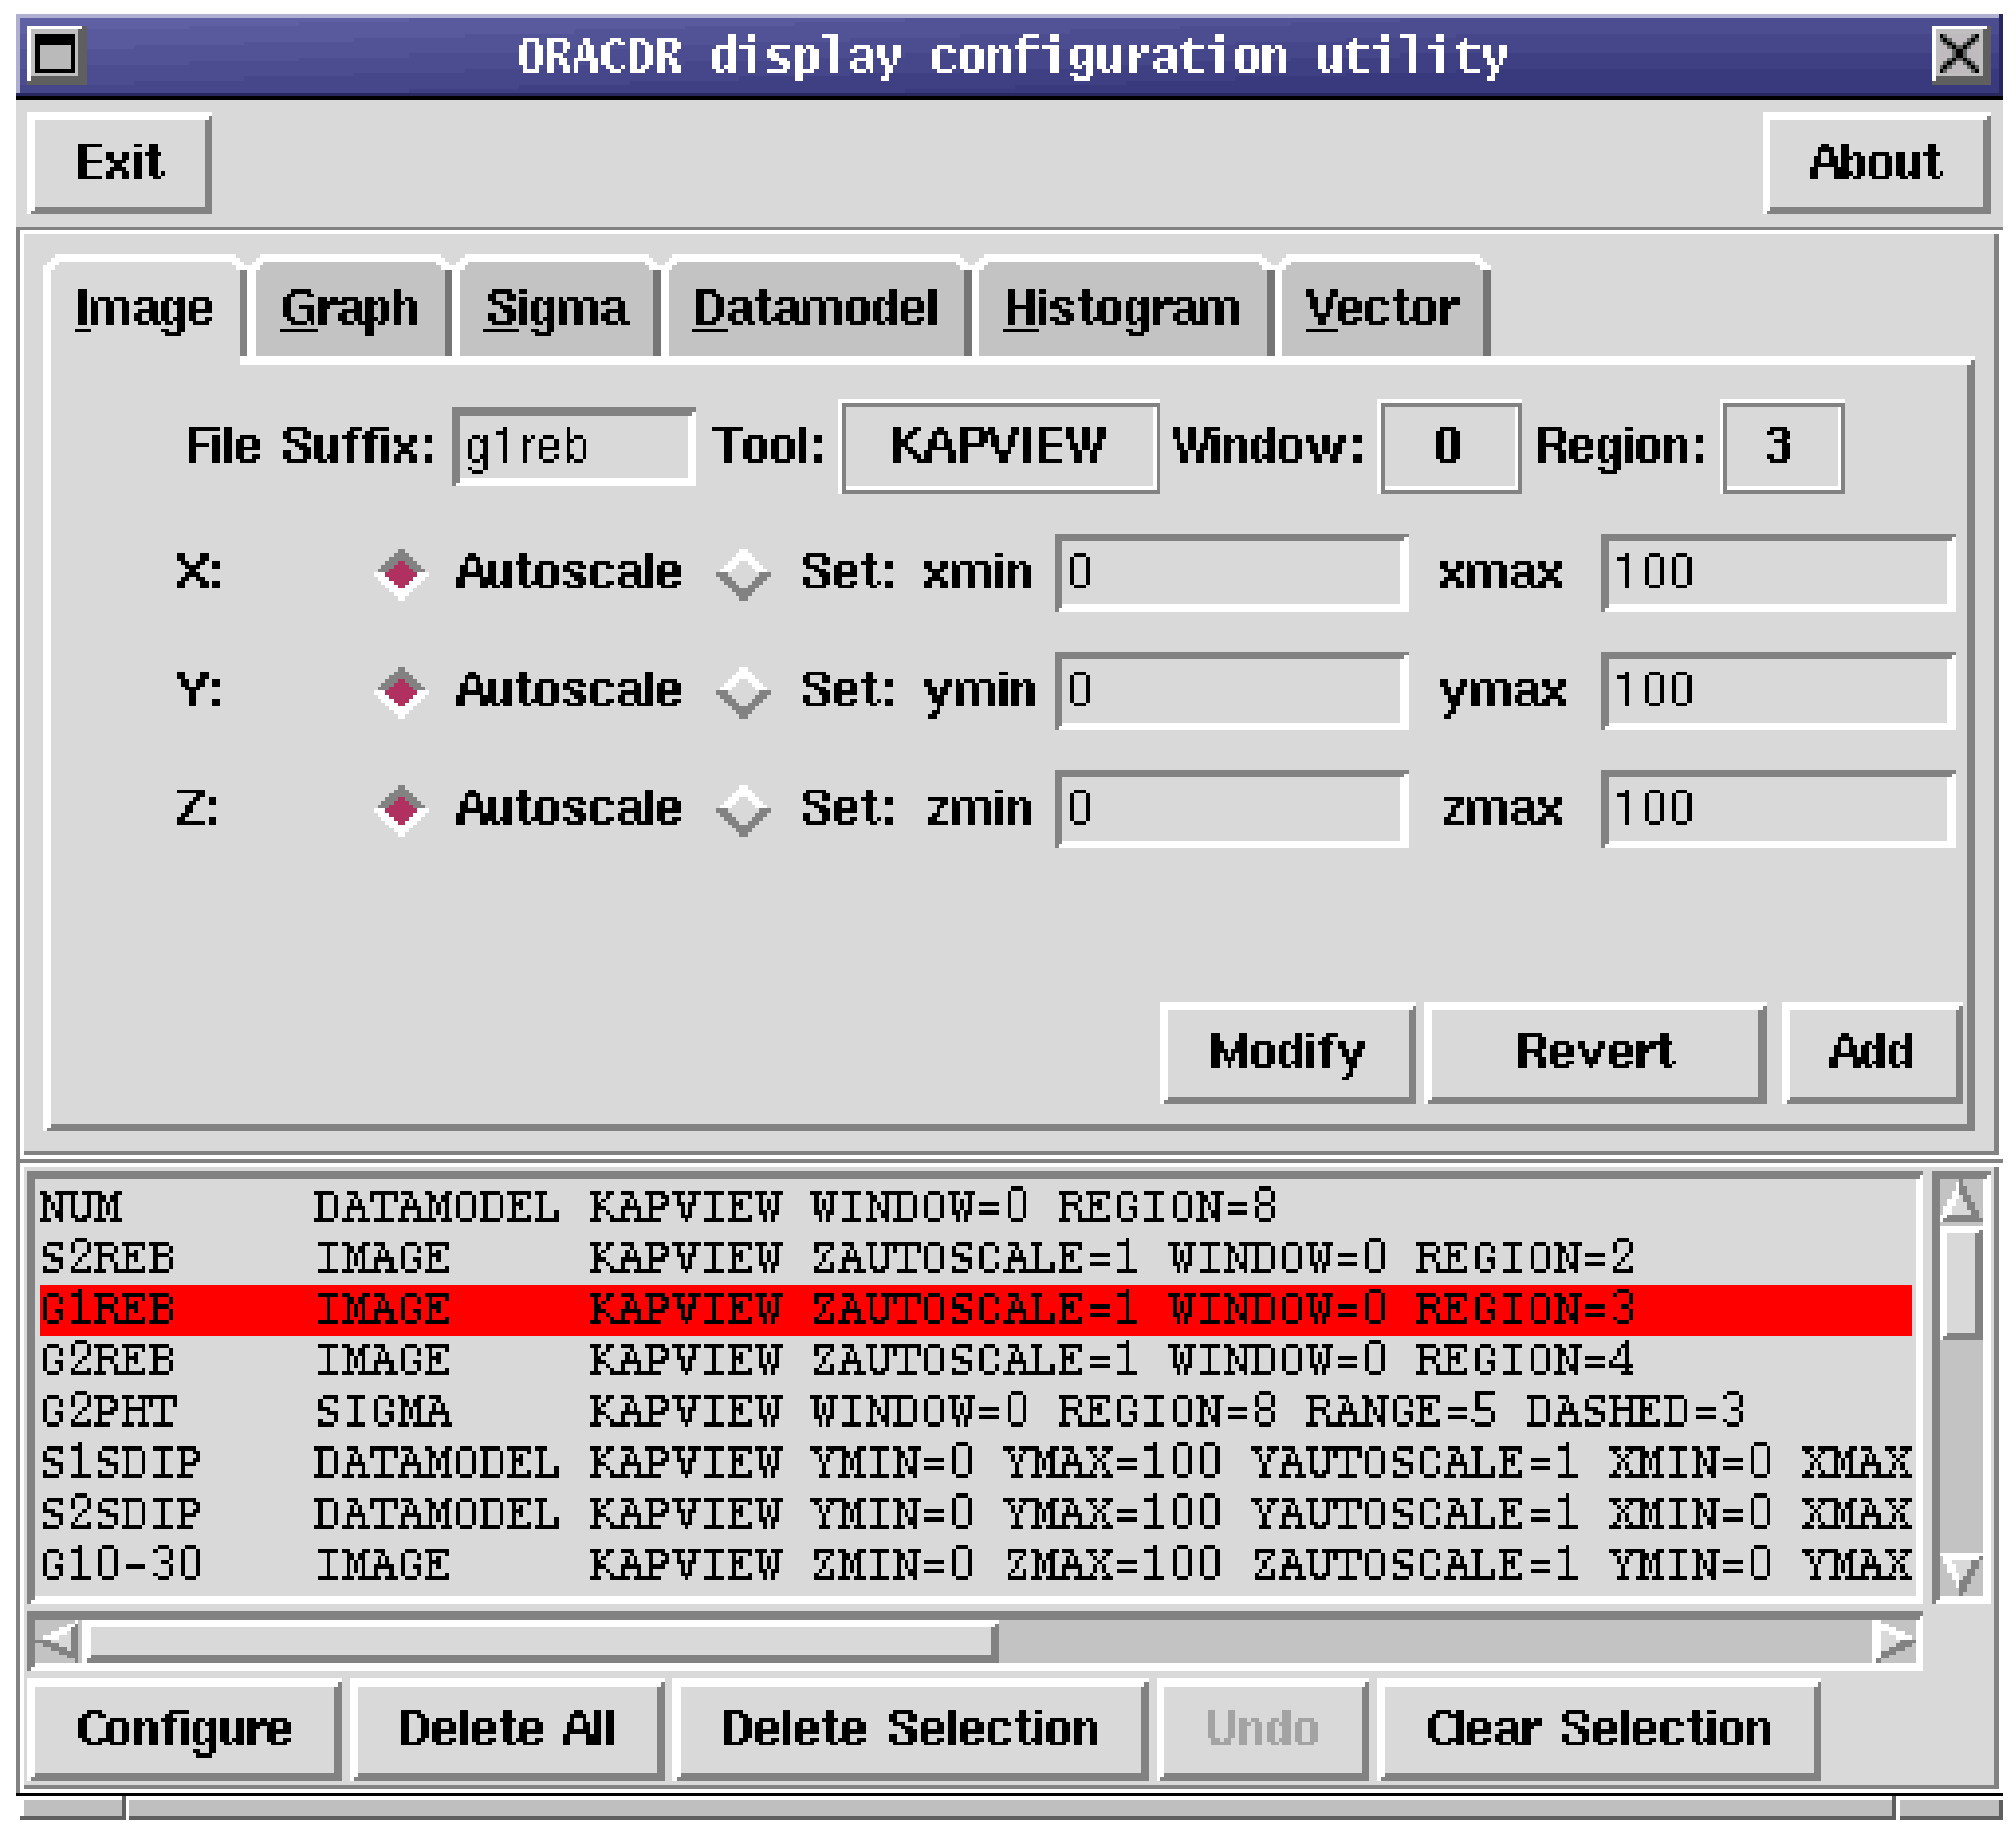
\includegraphics[width=\textwidth]{sun230_disp.eps}
\caption{The \texttt{oracdisp} display configuration tool}
\end{figure}


\subsubsection*{How the pipeline displays}
\index{How the pipeline displays}

The {\em disp.dat\/} file has a series of entries consisting of a line
each. Each line has a series of space-separated items.  All but
the first item, the suffix, use the keyword=value syntax.

These items are:

\begin{description}

\item[suffix]
\index{suffix@suffix}
\hfil\\
A file suffix representing a particular step of the data reduction
process as designated by that instrument's file naming convention. For
example, for UFTI data ``dk'' states what to do with a file called
{\tt f19990330\underscore{}00042\underscore{}dk.sdf\/}. Many entries may be made for a particular
suffix. The following special conventions are used: NUM describes a
file ending in just an observation number (usually representing raw
data). For instruments that have multiple data arrays in a single data
frame, S2$<$suffix$>$ (e.g. S2dk) represents the second data array in the
frame with the \underscore{}dk suffix.

\item[tool]
\index{tool@tool}
\hfil\\
A display tool such as {\tt Gaia} or \kapview\ (the latter being a collective
term for various \Kappa\ display tasks). The tools available are
determined by the display type (q.v.) selected.

\item[type]
\index{type@type}
\hfil\\
A display type such as graph, image, contour etc. These vary according 
to the tool selected.   The following types are available.  The tools
which support the given display type are listed in parentheses.

\begin{description}

\item[contour (\kapview)]
\index{contour (KAPVIEW)@contour ({\tt KAPVIEW})}
\hfil\\
Plots a contour plot.

\item[datamodel (\kapview)]
\index{datamodel (KAPVIEW)@datamodel ({\tt KAPVIEW})}
\hfil\\
Displays data (as points) with a model overlaid.

\item[graph (\kapview, \textsc{p4})]
\index{graph (KAPVIEW, P4)@graph ({\tt KAPVIEW}, {\tt P4})}
\hfil\\
Plots a line graph such as a spectrum.

\item[histogram (\kapview)]
\index{histogram (KAPVIEW)@histogram ({\tt KAPVIEW})}
\hfil\\
Plots a line graph such as a spectrum.

\item[image (\gaia, \kapview, \textsc{p4})]
\index{image (GAIA, KAPVIEW, P4)@image ({\tt GAIA}, {\tt KAPVIEW}, {\tt P4})}
\hfil\\
Displays an image.

\item[sigma (\kapview)]
\index{sigma (KAPVIEW)@sigma ({\tt KAPVIEW})}
\hfil\\
Draws a scatter plot with a Y range of +/- N standard deviations.

\item[vector (\kapview)]
\index{vector (KAPVIEW)@vector ({\tt KAPVIEW})}
\hfil\\
Displays an image and vectors (e.g. polarimetry data).

\end{description}

\item[window]
\index{window@window}
\hfil\\
The number of the window in which the display is to go. The value of
this is simply an identifier and does not presuppose order. If you ask 
for an image display to go to window 2 and you have configured no
displays to go to windows 0 and 1 then you will only get one window on 
your screen. If you then configure a histogram display to go to window 
2 it will go to the same window whereas if you configure it to go to
window 1 (or 5 or 9 or anything else besides 2) it will end up in its
own window. Note that no windows are launched until they are
required.

\item[region]
\index{region@region}
\hfil\\
For device tools that support it, region addresses the parts of a
window where a display ends up. For KAPVIEW, these are: whole screen
(0), top left quarter (1), top-right quarter (2), bottom-left quarter
(3), bottom-right quarter (4), left half (5), left right (6), top half 
(7), bottom half (8).  Defaults to 0.

\item[xautoscale]
\index{xautoscale@xautoscale}
\hfil\\
Specifies whether or not to use a section of the data frame.  If set to
1, meaning true, the whole X axis is used.  If set to 0, the pixel limits
are specified by keywords xmin and xmax.  The default is 1.

There are corresponding autoscaling keywords for higher dimensions
named yautoscale, 3autoscale, 4autoscale etc.

\item[xmin, xmax]
\index{xmin, xmax@xmin, xmax}
\hfil\\
The X-axis pixel limits of the data to be displayed when xautoscale=1.
xmin should be less than or equal to xmax.  There are corresponding
pixel-range keywords for higher dimensions: ymin and ymax, 3min and
3max, 4min and 4max etc. when autoscaling on the corresponding axis is
disabled.

\item[zautoscale]
\index{zautoscale@zautoscale}
\hfil\\
Set to 1 meaning true, this scales this requests that the data are
scaled automatically between the data range.  In the case of images on
\gaia\ the cut is at the 95 percentile.  When zautoscale is 0, the
scaling is between the limits defined by keywords zmin and zmax.
Defaults to 1 if absent.

\item[zmin, zmax]
\index{zmin, zmax@zmin, zmax}
\hfil\\
When zautoscale is 1, these specifiy the lower and higher 
scaling limits for the data values.

\end{description}

\subsubsection*{The order of play}
\index{order of play}

Every time a primitive creates a meaningful file with a particular suffix, it
sends a display request to the display system. For example, suppose the
primitive that performs dark subtraction creates a frame called {\tt
f19990330\underscore{}00042\underscore{}dk.sdf\/} and then asks the display
system to display it. The display system consults the {\em disp.dat\/} file
for a dk entry. If no such entry is found, the display request is ignored and
nothing happens. If one or more entries are found the display system proceeds
to honour the request. If the {\em disp.dat\/} entry specifies a particular
tool and/or window, the display system checks to see if they exist already and
if not, stars them. Then it displays the data with the appropriate parameters.


%% ORACDRDOC_HOWTO:Calibrating
% LaTeX document produced by pod2latex from "Calibrating.pod".
% The followings need be defined in the preamble of this document:
%\def\C++{{\rm C\kern-.05em\raise.3ex\hbox{\footnotesize ++}}}
%\def\underscore{\leavevmode\kern.04em\vbox{\hrule width 0.4em height 0.3pt}}
%\setlength{\parindent}{0pt}

\section{Calibrating\xlabel{calibrating}}
\index{CALIBRATING}

\oracdr\ has a totally flexible system for controlling the automatic
selection of calibration frames. This section describes how it works and
how to override it 

\subsubsection*{What happens}
\index{What happens}

The type of calibrations used depend, obviously, on the instrument and
the data reduction recipes used. Typically there are three kinds of
calibration frames:

\begin{itemize}

\item
Library frames provided by the observatory (bad pixel masks, rotation
transformations, etc). These are maintained by the instrument
scientist as appropriate. They are located in {\tt ORAC\char`\_DATA\char`\_CAL}.

\item
Nightly frames that are generated during observing. The may be taken
in specific calibration observations, e.g. by taking a ``dark'' (at UKIRT)
or ``skydip'' (at JCMT) frames. They might also be generated from
actual observations of targets (such as ``sky flats'') or
calibration values (such as ``flux conversion factors'') calculated
as part of a recipe. These are located in {\tt ORAC\char`\_DATA\char`\_OUT}.

\item
``Rule'' files that contain the rules for what constitutes an
appropriate calibration frame. These are located in {\tt ORAC\char`\_DATA\char`\_CAL}.

\end{itemize}

\oracdr\ treats the first two kinds rather differently. 

Library frames reside {\tt ORAC\char`\_DATA\char`\_CAL} and their selection is hardwired
either in the instrument class or in a DR primitive. The users are
unlikely to be concerned with them unless they want to override them
with their own.

Nightly frames are handled in a more complicated way. A DR recipe that
generates a calibration frame is responsible for filing it with the
pipeline. The pipeline will hand it back to recipes that require
calibration recipes according to a set of rules that are defined
on a per-instrument basis by the \oracdr\ infrastructure as well
as a per-frame basis by the calibration rules files.

\subsubsection*{Finding calibration frames}
\index{Finding calibration frames}

When a frame is reduced and files as a calibration, it is added to an
index file located in {\tt ORAC\char`\_DATA\char`\_OUT} named after the type of
calibration, e.g., dark frames are filed in {\em index.dark\/}. When the
pipeline is run up and needs a calibration frame but has not been
asked to reduce one in that session it will look in the index files
for one that may have been reduced at a previous time. 

If the pipeline is unable to find a suitable calibration it will
complain vociferously and exit. This may seem extreme, but remember
that \oracdr\ is designed for online use at an observatory. If an
observer has not taken appropriate calibrations, we wish to point
it out to them in the strongest terms because we do not want them
to end up with un-reduceable data.

\subsubsection*{Overriding defaults}
\index{Overriding defaults}

You can override the pipeline's selection of calibration frame by
using the \oracdr\ {\tt -calib} command line option. Use this override
judiciously, as in general the pipeline does a fine job.

For more information on selection of calibration frames, consult the
user guide for your instrument.


%% ORACDRDOC_HOWTO:ShellVariables
% LaTeX document produced by pod2latex from "ShellVariables.pod".
% The followings need be defined in the preamble of this document:
%\def\C++{{\rm C\kern-.05em\raise.3ex\hbox{\footnotesize ++}}}
%\def\underscore{\leavevmode\kern.04em\vbox{\hrule width 0.4em height 0.3pt}}
%\setlength{\parindent}{0pt}

\section{Shell Variables\xlabel{shell_variables}}
\index{SHELLVARIABLES}

This section describes the complete list of environment variables
used by the pipeline.

\subsection*{Complete variable list}
\index{Complete variable list}

\oracdr\ uses a number of environment variables for configuration.

\subsubsection*{User variables}
\index{User variables}

Users may need to change the following variables before using the
software. 

\begin{description}

\item[{\tt ORAC\char`\_DATA\char`\_ROOT}]
\index{ORAC_DATA_ROOT@{\tt ORAC\char`\_DATA\char`\_ROOT}}
\hfil\\
Location of the raw and reduced data directories if it confirms with
the naming convention for the instrument. Should be set before the
instrument startup script, which uses this variable to set
{\tt ORAC\char`\_DATA\char`\_IN} and {\tt ORAC\char`\_DATA\char`\_OUT}.

\item[{\tt ORAC\char`\_DATA\char`\_IN}]
\index{ORAC_DATA_IN@{\tt ORAC\char`\_DATA\char`\_IN}}
\hfil\\
Actual location of raw data files. Should be set after the instrument
startup script. 

\item[{\tt ORAC\char`\_DATA\char`\_OUT}]
\index{ORAC_DATA_OUT@{\tt ORAC\char`\_DATA\char`\_OUT}}
\hfil\\
Actual location of reduced data files. This is also the working
directory of the pipeline. Should be set after the instrument startup
script.

\item[{\tt ORAC\char`\_CAL\char`\_ROOT}]
\index{ORAC_CAL_ROOT@{\tt ORAC\char`\_CAL\char`\_ROOT}}
\hfil\\
Directory where the instrument specific 

\item[{\tt ORAC\char`\_DATA\char`\_CAL}]
\index{ORAC_DATA_CAL@{\tt ORAC\char`\_DATA\char`\_CAL}}
\hfil\\
Location of the calibration files for the instrument. Set by the
instrument startup script to \\
{\tt ORAC\char`\_CAL\char`\_ROOT/<instrument>}.

\item[{\tt ORAC\char`\_RECIPE\char`\_DIR}]
\index{ORAC_RECIPE_DIR@{\tt ORAC\char`\_RECIPE\char`\_DIR}}
\hfil\\
Location of user-defined recipes. These supersede any identically
names ones in \\
{\tt ORAC\char`\_DIR/recipes/<instrument>}.

\item[{\tt ORAC\char`\_PRIMITIVE\char`\_DIR}]
\index{ORAC_PRIMITIVE_DIR@{\tt ORAC\char`\_PRIMITIVE\char`\_DIR}}
\hfil\\
Location of user-defined primitives. These supersede any identically
names ones in \\
{\tt ORAC\char`\_DIR/primitives/<instrument>}.

\end{description}

\subsubsection*{System variables}
\index{System variables}

Starlink and JAC users should not redefine these variables under
normal circumstances because they are correctly set by their user
logins. They are included here for reference only.

\begin{description}


\item[{\tt ORAC\char`\_DIR}]
\index{ORAC_DIR@{\tt ORAC\char`\_DIR}}
\hfil\\
The location of the \oracdr\ software directory. This is normally set
by a login script. 

\item[{\tt ORAC\char`\_INSTRUMENT}]
\index{ORAC_INSTRUMENT@{\tt ORAC\char`\_INSTRUMENT}}
\hfil\\
The instrument under whose environment \oracdr\ should run. Normally
this is set by the appropriate instrument script in {\tt ORAC\char`\_DIR/etc/}

\item[{\tt ORAC\char`\_PERL5LIB}]
\index{ORAC_PERL5LIB@{\tt ORAC\char`\_PERL5LIB}}
\hfil\\
The location of the \oracdr\ perl libraries. These are normally in
{\tt ORAC\char`\_DIR/lib/perl5}.

\item[{\tt ORAC\char`\_PERSON}]
\index{ORAC_PERSON@{\tt ORAC\char`\_PERSON}}
\hfil\\
The address of the JAC contact who supports \oracdr\ for
{\tt \$ORAC\char`\_INSTRUMENT}. This is used in the splash screen.

\item[{\tt ORAC\char`\_LOOP}]
\index{ORAC_LOOP@{\tt ORAC\char`\_LOOP}}
\hfil\\
The default type of looping scheme that should be used for online
reduction of {\tt ORAC\char`\_INSTRUMENT}. This  is used in the splash screen. 

\item[{\tt ORAC\char`\_SUN}]
\index{ORAC_SUN@{\tt ORAC\char`\_SUN}}
\hfil\\
The Starlink User Note number that documents the data reduction for
{\tt ORAC\char`\_INSTRUMENT}. This  is used in the splash screen. 

\end{description}

%% ORACDRDOC_BIN:oracdisp
% LaTeX document produced by pod2latex from "oracdisp.pod".
% The followings need be defined in the preamble of this document:
%\def\C++{{\rm C\kern-.05em\raise.3ex\hbox{\footnotesize ++}}}
%\def\underscore{\leavevmode\kern.04em\vbox{\hrule width 0.4em height 0.3pt}}
%\setlength{\parindent}{0pt}

\section{ORACDISP\xlabel{oracdisp}}
\index{ORACDISP}


Controls the display environment used by \oracdr. This routine
can be used to edit the current environment and add display directives
to the current environment.

\begin{verbatim}
  oracdisp [-h] [-v] [-in=file] [-out=file]
\end{verbatim}


\subsection*{Arguments}
\index{ARGUMENTS}

The following command line arguments are recognised by {\tt oracdisp}:

\begin{description}

\item[{\bf -h}]
\index{-h@{\bf -h}}

Prints help information describing the arguments.

\item[{\bf -v}]
\index{-v@{\bf -v}}

Prints version number information.

\item[{\bf -in}]
\index{-in@{\bf -in}}

Used to modify the name of the input display definition file.
Default is {\em disp.dat\/}. Do not modify if used in conjunction with
\oracdr.

\item[{\bf -out}]
\index{-out@{\bf -out}}
\hfil\\
Used to modify the name of the output display definition file.
Default is {\em disp.dat\/}. Do not modify if used in conjunction with
\oracdr.

\end{description}

\subsection*{Notes}
By default, {\tt oracdisp} manipulates a file called {\em disp.dat\/}
in the {\tt ORAC\char`\_DATA\char`\_OUT} directory. Do not modify the name of this
file for use with \oracdr\ (since \oracdr\ is expecting a file
called {\em disp.dat\/} in {\tt ORAC\char`\_DATA\char`\_OUT}).


%% ORACDRDOC_BIN:oracdr_nuke
% LaTeX document produced by pod2latex from "oracdr_nuke.pod".
% The followings need be defined in the preamble of this document:
%\def\C++{{\rm C\kern-.05em\raise.3ex\hbox{\footnotesize ++}}}
%\def\underscore{\leavevmode\kern.04em\vbox{\hrule width 0.4em height 0.3pt}}
%\setlength{\parindent}{0pt}

\section{ORACDR\underscore{}NUKE\xlabel{oracdr_nuke}}
\index{ORACDR\underscore{}NUKE}

Attempt to kill all \oracdr\ related processes and shared memory that
can be found and that are associated with the current user.

\subsection*{Notes}
\begin{itemize}

\item
All shared memory owned by the current user is removed even if
it is not directly associated with an \oracdr\ process.

\item
Will not attempt to remove shared memory owned by another user.

\item
Will attempt to kill processes owned by other users even though
this will not succeed unless the user has special privilege.

\item
Does not attempt to clear out ADAM\underscore{}USER directories. This is not
normally a problem for \oracdr\ since each \oracdr\ process works
in a different ADAM\underscore{}USER directory.

\end{itemize}


% ? End of main text
\end{document}
